In this section we will review the way the pronunciation scoring system works
and explain the concepts and techniques on which it is based. The diagram bellow
shows the overall architecture of the system:

~

\begin{figure}[H]
	\centering
	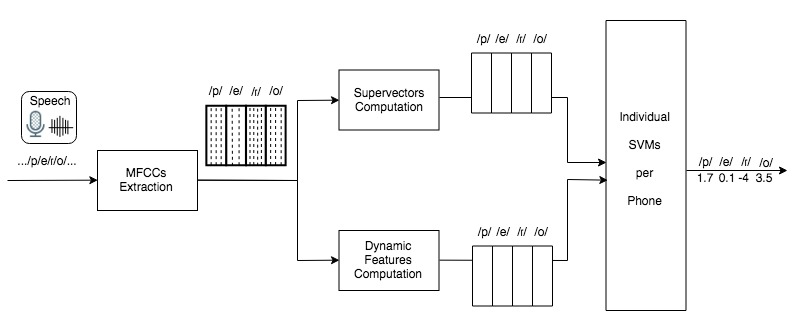
\includegraphics[width=0.9\textwidth]{files/figures/method/general-structure-v2.jpg}
	\caption{General System Architecture}
	\label{fig:methodGeneralArchitecture}
\end{figure}

Given a test instance, the objective is to compute a score for each phone that
is uttered in that instance. In order to do so, the flow goes as follows:

\begin{enumerate}

 \item The first step is to calculate the audio features from the recordings.
 This is done in order to summarize the signal information
 in a measurable way through numeric values. The chosen features
 are the \textit{Mel Frecuency Cepstral Coefficients} (MFCCs) because they are one of the
 most standard and widely-spread features in the speech processing field.

 \item The MFCCs are then splitted in segments according to the phones to which they
 belong. Each segment is at the same time divided in frames, that represent short
 intervals where the audio signal is not supposed to be changing so much.

 \item MFCCs of each instance of the phone present in the utterance
 are then used to compute the more complex features
 on which the SVMs operates. Supervectors are the base and proven to work features,
 while the Dynamic Features are the experimental features to be studied.
 There is an individual classifier for each of the phones.

 \item Finally an individual score is obtained for each of the phones present in the
 utterance. Scores with positive sign corresponds to correctly pronounced instances of the phone
 while scores with negative sign corresponds to mispronunciations. The magnitude of the score
 is associated with how well or bad the phone is pronounced.
 The bigger the magnitude of the score, the better the pronunciation when the sign is positive
 and the worst the mispronunciation when the sign is negative.

\end{enumerate}

% Given a phone utterance the objective is to determine wheter or not it was correctly
% pronounced, with the possibility of returning
% a more specific value that measures how well or bad that uttered phone
% was pronounced.

% The input data consists of recordings of read
% speech that belongs to nonnative speakers with different proficiency levels.
% The phone is the unit of analysis, so the first step is extracting the information
% for each phone instance in the utterances.  In order to do so,
% an HMM-based (Hidden Markov Model) recognition system is used to obtain the phonetic
% segmentations of the utterances, and these segmentations along with an external tool
% called \emph{Kaldi} are then used to extract the
% acoustic features for each phone. At the same time, manual transcriptions of profesional
% annotators are used to obtain labels for each instance. A label has two possible values (0 or 1),
% and determines if a given instance of a phone was correctly or incorrectly pronounced.

% After that, labels and features are used to prepare a dataset: training and test sets. The first
% one is used to explore different models and find the parameters that lead to the
% best possible configurations.
% Finally, after picking the model with the best performance it is tested against the heldout data
% and the results are analyzed.

